\section{Context} \label{sec:intro-context}
While \textit{artificial intelligence} (AI) - as a field - has existed for nearly seventy years \citep{moor2006dartmouth}, the concept of artificial intelligence dates back at least to ancient Greece.  
In early times, artificial intelligence, embodied in the dream of mechanical men, was part of the domain of myth; in the twentieth century, of that of science.  
During this last decade, artificial intelligence is no longer part of a single, specific domain, as it has materialised from Man's imagination, broken out of laboratories and has been given license to act in the world at large.

Artificial intelligence and specifically \textit{machine learning}, the branch of AI that specialises in creating computer systems able to learn their programming from real-world examples instead of having to be explicitly coded by a human, have in the last two decades seen extraordinary success\footnote{See \citet{shalev2014understanding} for an introduction to machine learning and Figure \ref{fig:ai-overview} to get an overview of the field of AI.}.
No sector of our economy has been left untouched by the recent and rapid rise of machine learning, which has been enabled by the rediscovery of neural networks, the availability of big data and increased access to parallel computing power\footnote{A compelling talk, explaining the recent rise of ML, by AI pioneer Geoff Hinton can be found at \url{https://www.youtube.com/watch?time_continue=1&v=izrG86jycck}.}.
Fields as diverse and critical as are government, healthcare, finance and bioinformatics have been revolutionised and the opportunity has been opened for new sectors - such as self-driving vehicles - to appear\footnote{For an overview of the impacts of AI on current society and labour market see \citet{schwab2017fourth}.}.
The increasing reliance of our civilisation on ever more complex machine learning-driven algorithms can only make us more worried about the ethical problems posed by such a series of circumstances.  
Our society has only very recently been confronted with the dilemma of assigning responsibility when a driverless car causes the death of a person\footnote{\url{https://www.nytimes.com/interactive/2018/03/20/us/self-driving-uber-pedestrian-killed.html}}.
This moral issue is only the tip of the iceberg, even when focusing exclusively on the automotive industry.  
As an increasing number of decisions are made in an automated way, with many of them significantly impacting both individuals and society at large, it is natural to stop and wonder which characteristics are desirable in the systems tasked with giving us these verdicts.  

 \begin{figure}[htbp]
\centerline{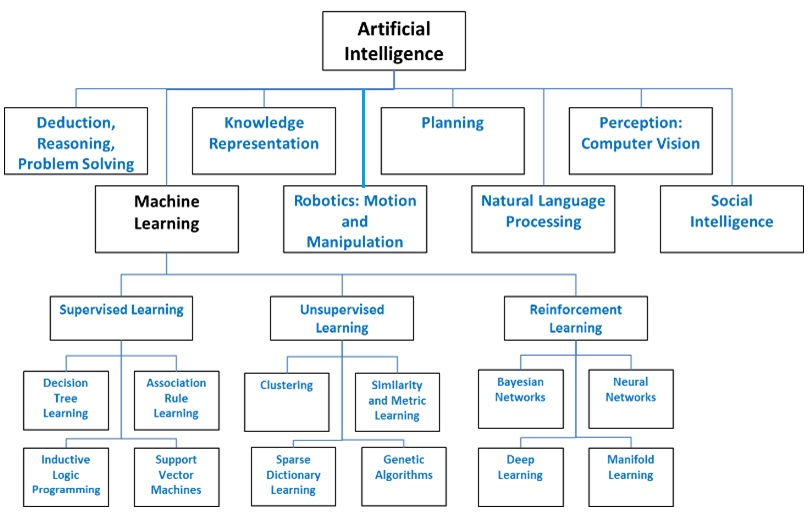
\includegraphics[width=\textwidth]{introduction/images/ai-overview}}
\caption{Dendrogram showing an overview of the field of AI with the position of ML emphasised [\href{https://tu-dresden.de/ing/informatik/ressourcen/dateien/studium/lehrangebot/forschungslinie_einfuehrung_in_die_forschung/2017/2017-04-03-FG-KI.pdf}{Sebastian Rudolph}].}
\label{fig:ai-overview}
\end{figure}

\textit{Explainable AI} (xAI) is the sub-field of artificial intelligence that ideally should be found at the intersection between computer science, social sciences and philosophy and that should aim to define the desiderata of artificially intelligent systems and to develop methods to achieve these.
For example, how should a self-driving car behave when confronted with a real-world predicament analogous to the classic trolley problem - a situation where each course of action is liable to cause harm?  
On what basis should a person be denied a mortgage, access to university or a job interview?  How can we be sure that the bias in the system is reduced to an acceptable level?  How do we even define if the system is behaving morally?  Would it currently be feasible for a person  to appeal an automated decision they feel they had been harmed by?\footnote{For an overview of AI ethics see \citet{Bostrom2011}.}
The main strategy developed in order to achieve these goals is for the systems in question to be somehow made \textit{explainable}. 
The problems in this process start at the very first step, given that within the xAI community, as noted by \citet{Doran2018}, there is currently no unanimously agreed upon definition of \textit{explainability} and consequently of the best way to achieve it in real systems.
The review carried out in Section \ref{sec:explainability} highlights one of the fundamental problems of the field of xAI: that all researchers within the community claim their methods to be \enquote{explainable}, but very few justify this with reasons grounded in the real world (as best summarised in the popular paper \citep{Lipton2016}).

To solve this conundrum, various authors have tried to define taxonomies which classify systems based on their characteristics and how these relate to their perceived explainability.
One of the most compelling of these is that proposed by \citet{Doran2018} and shown in Figure \ref{fig:xai-systems-taxonomy}.
The highest level in this classification is occupied by \textit{explainable systems} i.e., those that emit explicit, human-understandable reasonings.
This category appears somewhat nebulous in light of the previous paragraph: how should an explainable system be recognised if there is no good definition of explanation?
A less elaborate, but still conceptually sound taxonomy is the one proposed by \citet{mittelstadt2019explaining} who propose to classify systems based on the source, or \textit{locus}, of their explainability.
In this classification, models may be \textit{ante-hoc} or \textit{post-hoc} explainable; the former identifies systems whose explainability stems from some internal, inherent characteristic while the latter those whose source of explainability is to be found in some external behaviour, for example in the emission of extra symbols along the output.
The two taxonomies are somewhat overlapping - even though the latter by \citet{mittelstadt2019explaining} does not consider \textit{opaque} systems; the two classifications could be put into relationship by identifying \textit{interpretable} with \textit{ante-hoc} and \textit{comprehensible} together with \textit{explainable} with \textit{post-hoc}.
A third orthogonal classification forwarded by \citet{doshi2017towards} addresses how to evaluate the quality of an explanation.
The first two taxonomies will be presented in more detail in Section \ref{sec:explainability} while the last in Section \ref{sec:evaluation-of-explainability}.

\begin{figure}[htbp]
\centerline{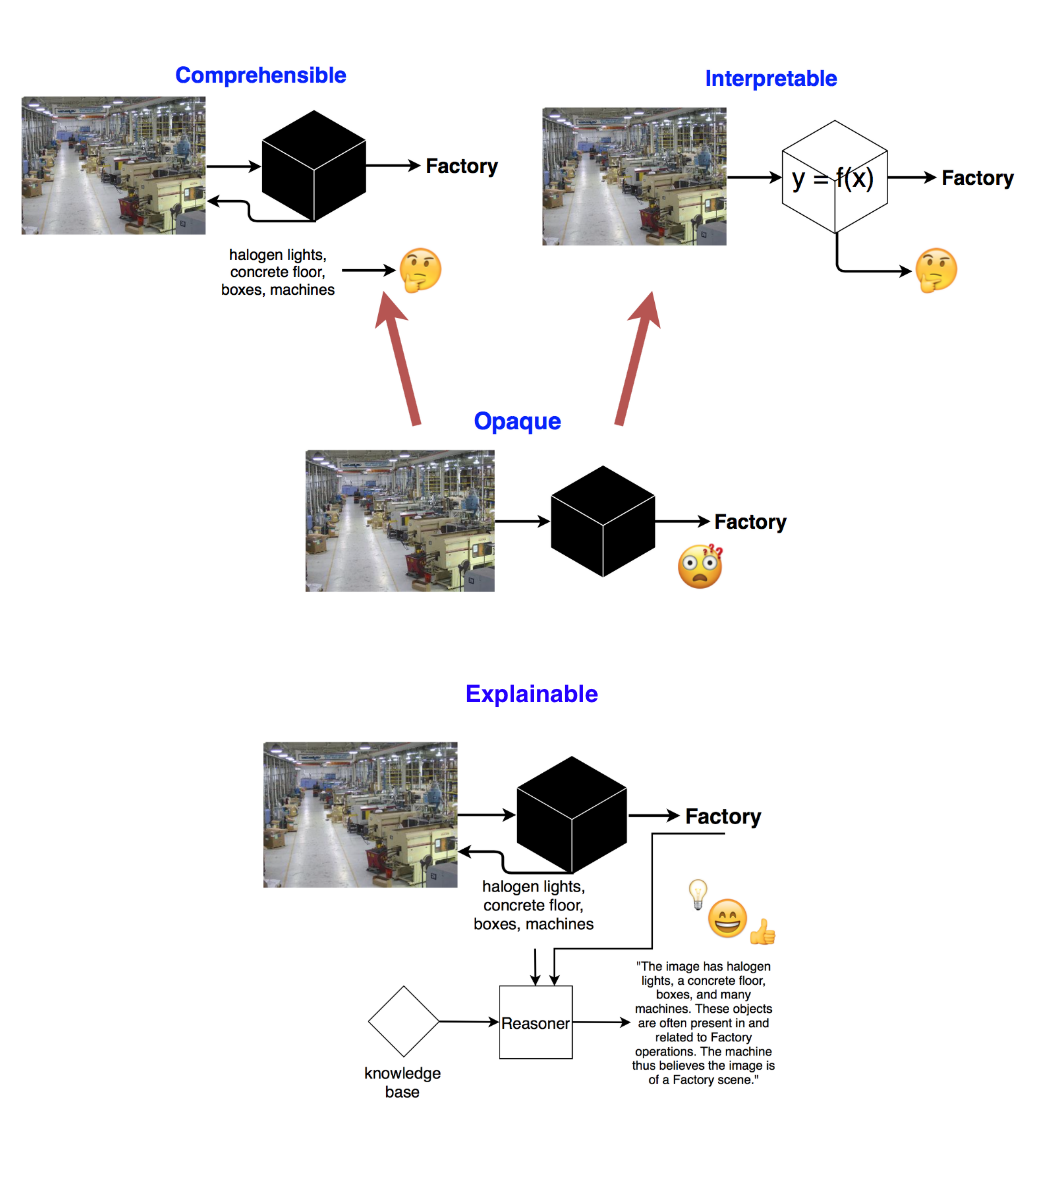
\includegraphics[width=0.9\textwidth]{introduction/images/xai-systems-taxonomy}}
\caption{The relationship between \textit{opaque}, \textit{interpretable},  \textit{comprehensible} and \textit{interpretable} systems [adapted from \citep{Doran2018}].}
\label{fig:xai-systems-taxonomy}
\end{figure}

The purpose of this brief introduction to explainable artificial intelligence, is to help in understanding that many of the problems that the field aims to tackle are hard \textit{per-se} and may not have a unique optimal solution.  
This is because such issues are not only engineering problems, but exist at the intersection between man and machine and as such cannot be solved using only engineering methods\footnote{This is what is meant by \citet{doshi2017towards} when they talk about \enquote{incompleteness in the problem formalization}.}.  
This lack of awareness for the centrality of the human element of an explanation is one of the main pitfalls of the xAI community, since most of its researchers come from the \textit{hard-science domains} of computer science, mathematics and statistics. 
There is little hope of defining the desiderata for intelligent systems without the guidance that can only come from philosophy, because of its millennia-long tradition in dealing with ethical issues.  
There is also no way to satisfactorily move towards and evaluate these desiderata without resorting to the well-established literature and methods of the social sciences\footnote{For a good example of how this may work, see \citet{stumpf2009interacting}.}, as the human element is inherent in any explanation. 
An attempt to define how a computer should relate itself to its user could be assimilated with the notion of \enquote{reinventing the wheel}, as the field of human computer interaction has many such techniques already. 
Although an endeavour still pursued by many xAI researchers, it should be clear that when the human - and particularly the ethical - domain are part of the equation, it is impossible \textit{by definition} to find an optimal and unique solution\footnote{See the concept of \enquote{wicked problem} in \citep{Rittel1973}.}.

Effectively, the biggest gap that can be identified is a dearth of explainability methods that have been validated not only by domain experts, but even by real humans.
Many researchers seem content with claiming \textit{formal explainability} and neglect the human element of the explanation.
An explanation, by its vert nature, involves an \textit{explainer}, the machine, and an \textit{explainee}, us humans.
Up till now, it seems that xAI is content with only explaining the machine but, in doing so, overlooks the fact that it may be offering the users no explanation at all\footnote{See \citet{mittelstadt2019explaining} for a critique of the field of xAI, based on this lack of awareness.}.